%%%%%%%% ICML 2026 EXAMPLE LATEX SUBMISSION FILE %%%%%%%%%%%%%%%%%

\documentclass{article}

% Recommended, but optional, packages for figures and better typesetting:
\usepackage{microtype}
\usepackage{graphicx}
\usepackage{subcaption}
\usepackage{booktabs} % for professional tables

% hyperref makes hyperlinks in the resulting PDF.
% If your build breaks (sometimes temporarily if a hyperlink spans a page)
% please comment out the following usepackage line and replace
% \usepackage{icml2026} with \usepackage[nohyperref]{icml2026} above.
\usepackage{hyperref}


% Attempt to make hyperref and algorithmic work together better:
\newcommand{\theHalgorithm}{\arabic{algorithm}}

% Use the following line for the initial blind version submitted for review:
\usepackage{icml2026}

% For preprint, use
% \usepackage[preprint]{icml2026}

% If accepted, instead use the following line for the camera-ready submission:
% \usepackage[accepted]{icml2026}

\usepackage{amsmath}
\usepackage{amssymb}
\usepackage{mathtools}
\usepackage{amsthm}


% if you use cleveref..
\usepackage[capitalize,noabbrev]{cleveref}

%%%%%%%%%%%%%%%%%%%%%%%%%%%%%%%%
% THEOREMS
%%%%%%%%%%%%%%%%%%%%%%%%%%%%%%%%
\theoremstyle{plain}
\newtheorem{theorem}{Theorem}[section]
\newtheorem{proposition}[theorem]{Proposition}
\newtheorem{lemma}[theorem]{Lemma}
\newtheorem{corollary}[theorem]{Corollary}
\theoremstyle{definition}
\newtheorem{definition}[theorem]{Definition}
\newtheorem{assumption}[theorem]{Assumption}
\theoremstyle{remark}
\newtheorem{remark}[theorem]{Remark}

% Todonotes is useful during development; simply uncomment the next line
%    and comment out the line below the next line to turn off comments
%\usepackage[disable,textsize=tiny]{todonotes}
\usepackage[textsize=tiny]{todonotes}

% The \icmltitle you define below is probably too long as a header.
% Therefore, a short form for the running title is supplied here:
\icmltitlerunning{Detecting hidden chain-of-thought in LLMs}

\begin{document}

\twocolumn[
  \icmltitle{Detecting hidden chain-of-thought in large language models with linguistic, behavioral, and mechanistic indicators}

  % It is OKAY to include author information, even for blind submissions: the
  % style file will automatically remove it for you unless you've provided
  % the [accepted] option to the icml2026 package.

  % List of affiliations: The first argument should be a (short) identifier you
  % will use later to specify author affiliations Academic affiliations
  % should list Department, University, City, Region, Country Industry
  % affiliations should list Company, City, Region, Country

  % You can specify symbols, otherwise they are numbered in order. Ideally, you
  % should not use this facility. Affiliations will be numbered in order of
  % appearance and this is the preferred way.
  \icmlsetsymbol{equal}{*}

  \begin{icmlauthorlist}
    \icmlauthor{Firstname1 Lastname1}{equal,yyy}
    \icmlauthor{Firstname2 Lastname2}{equal,yyy,comp}
    \icmlauthor{Firstname3 Lastname3}{comp}
    \icmlauthor{Firstname4 Lastname4}{sch}
    \icmlauthor{Firstname5 Lastname5}{yyy}
    \icmlauthor{Firstname6 Lastname6}{sch,yyy,comp}
    \icmlauthor{Firstname7 Lastname7}{comp}
    %\icmlauthor{}{sch}
    \icmlauthor{Firstname8 Lastname8}{sch}
    \icmlauthor{Firstname8 Lastname8}{yyy,comp}
    %\icmlauthor{}{sch}
    %\icmlauthor{}{sch}
  \end{icmlauthorlist}

  \icmlaffiliation{yyy}{Department of XXX, University of YYY, Location, Country}
  \icmlaffiliation{comp}{Company Name, Location, Country}
  \icmlaffiliation{sch}{School of ZZZ, Institute of WWW, Location, Country}

  \icmlcorrespondingauthor{Firstname1 Lastname1}{first1.last1@xxx.edu}
  \icmlcorrespondingauthor{Firstname2 Lastname2}{first2.last2@www.uk}

  % You may provide any keywords that you find helpful for describing your
  % paper; these are used to populate the "keywords" metadata in the PDF but
  % will not be shown in the document
  \icmlkeywords{Machine Learning, ICML}

  \vskip 0.3in
]

% this must go after the closing bracket ] following \twocolumn[ ...

% This command actually creates the footnote in the first column listing the
% affiliations and the copyright notice. The command takes one argument, which
% is text to display at the start of the footnote. The \icmlEqualContribution
% command is standard text for equal contribution. Remove it (just {}) if you
% do not need this facility.

% Use ONE of the following lines. DO NOT remove the command.
% If you have no special notice, KEEP empty braces:
\printAffiliationsAndNotice{}
% Or, if applicable, use the standard equal contribution text:
% \printAffiliationsAndNotice{\icmlEqualContribution}

\begin{abstract}
Large language models (LLMs) can often correctly answer complex reasoning tasks without explicitly revealing the steps they take, raising a fundamental question: do these models internally perform multi-step CoT reasoning, or rely on direct-answer generation and pattern completion? Current approaches depend on surface-level linguistic cues that prior work has shown can be unfaithful, leaving no reliable method to detect implicit CoT when explicit reasoning is absent. We propose a framework that integrates linguistic, behavioral, and mechanistic interpretability signals, including token-level entropy, structured error patterns, and sensitivity to perturbations that disrupt intermediate dependencies, and a Hidden CoT Detection Score (HCDS) that quantifies whether neutral-prompt behavior aligns more closely with explicit CoT or with suppressed-CoT baselines. Evaluating Qwen3-4B Instruct and Thinking on GSM8K and StrategyQA, we find statistically significant positive HCDS for both models (GSM8K: +2.254 for Instruct and +0.479 for Thinking; StrategyQA: +1.871 for Instruct and +0.597 for Thinking). The Instruct result is our primary, cleanly-controlled hidden-CoT detection finding; the Thinking result we read with caution and reframe as evidence of prompt-invariance of reasoning traces, since Thinking emits $\sim$575 tokens of reasoning even under explicit answer-only directives and therefore lacks a clean no-CoT baseline. Anchor-suppression analysis further shows that the Thinking model distributes reasoning across many steps rather than concentrating it in critical anchors — though we caution that this signature is also consistent with attention-based anchor scoring biasing toward late-trace summary steps in long Thinking traces.
\end{abstract}

\section{Introduction}

Explicit Chain of Thought (CoT) prompting improves LLM performance and exposes interpretable reasoning steps~\citep{wei_chain--thought_2023}, but it is unclear whether models engage in latent or implicit CoT reasoning when users do not request step-by-step output. Current methods identify implicit CoT only through surface-level cues and behavioral patterns. These cues are correlational, not causal. Misidentifying such patterns as reasoning weakens interpretability and erodes user trust.

Models can plausibly produce forms of reasoning text that do not contribute to the final output~\citep{turpin_language_2023}. Distinguishing the two necessitates understanding whether the visible steps causally created the answer or simply accompany it. Output-only analysis cannot achieve this, because genuine step-by-step reasoning and post-hoc rationalization of an already-determined answer can yield the same surface text; the evidence that would separate them lies in the internal computation, not the output.

We reframe latent reasoning detection from a correlational analysis of model outputs into a behavioral identification problem. We propose the Hidden CoT Detection Score (HCDS), which quantifies the extent to which a model's neutral-prompt behavior resembles its explicit reasoning patterns. HCDS is computed by systematically comparing model behavior across explicit CoT, explicit no-CoT, and neutral prompts along three feature families: linguistic signals such as output length, token entropy, and step pattern similarity; behavioral signals such as latency per token, consistency across trials, and error-type clustering; and mechanistic signals from internal activations and attention patterns in open-weight models. The mechanistic signals additionally support targeted interventions that selectively disrupt internal dependencies, allowing us to evaluate whether specific steps causally contribute to the model's output rather than merely accompany it.

We evaluate HCDS on Qwen3-4B (Instruct and Thinking variants) using GSM8K and StrategyQA, comparing each model's behavior across the three prompt conditions. HCDS is significantly positive for both models under neutral prompting on both datasets (GSM8K: +2.254 for Instruct, p = 2.21e-10; +0.479 for Thinking, p = 2.06e-02; StrategyQA: +1.871 for Instruct, p = 3.53e-12; +0.597 for Thinking, p = 2.15e-03), indicating that neutral behavior aligns more closely with explicit CoT than with explicit no-CoT. The Instruct effect is robust across feature-ablation variants and across short, medium, and long questions; the Thinking effect is smaller and length-sensitive, weakening on medium-length questions where reasoning traces approach the generation cap. Anchor-suppression interventions further reveal that the Thinking model's explicit reasoning chains distribute causal load across many steps rather than concentrating in a few, an unexpected mechanistic finding the rest of the paper develops.


\section{Related Work}

A first line of related work asks whether visible chain-of-thought explanations faithfully reflect the computation that produces a model’s answer. \citet{turpin_language_2023} show that chain-of-thought explanations can be unfaithful, in the sense that models may produce plausible reasoning text that is not causally responsible for their final prediction. More recently, \citet{chen_reasoning_2025} test faithfulness through controlled prompt-hint interventions and show that reasoning traces do not always transparently reveal what the model used to reach its answer. These works motivate the central premise of our paper: output-only inspection is insufficient for determining whether reasoning is occurring internally. Our contribution differs in scope and objective. Rather than asking whether an explicit rationale is faithful, we ask whether latent reasoning is occurring at all under neutral prompting, and we address this question through a combination of behavioral and mechanistic signals rather than through rationale analysis alone.

A second line of work studies whether latent reasoning exists as a genuine internal phenomenon. \citet{lin_implicit_2025} argue that implicit reasoning in Transformers often emerges through shortcut learning and can fail to generalize when problem structure changes, suggesting that correct answers without explicit CoT need not imply robust reasoning. Concurrent work by \citet{he_reasoning_2026} provides mechanistic evidence that latent reasoning corresponds to steerable internal features, showing that reasoning behavior can be activated without explicit chain-of-thought prompting. These papers establish that latent reasoning is both real and difficult to interpret: it can exist as an internal computational mode, but may also be entangled with brittle heuristics. Our work differs by proposing a detection framework for identifying when such latent reasoning is being used at inference time, rather than studying how it emerges during training or how it can be induced through latent steering.

The work most closely related to our mechanistic component is \citet{bogdan_thought_2025}, who identify ``thought anchors'' --- reasoning steps within explicit CoT traces that have disproportionate influence on downstream generation. They propose black-box, attention-based, and causal attribution methods to determine which steps matter most within a visible reasoning chain. Our paper builds on this intervention logic but shifts the question from which explicit reasoning steps matter to whether reasoning is happening under neutral prompting at all. In our framework, anchor-based perturbation is not the end goal but one feature family within a broader hidden-CoT detection score. This difference is important: Bogdan et al. analyze the internal structure of explicit CoT, whereas we use related mechanistic tools to detect latent reasoning in the absence of explicit CoT.

\section{Background}

Our method builds on prior work in Transformer language models, chain-of-thought prompting, reasoning benchmarks, and causal interpretability. Because the goal of this paper is to detect hidden chain-of-thought reasoning rather than to elicit it directly, the relevant background is not only how reasoning prompts improve model performance, but also how internal computations in Transformer models can be analyzed through interventions.

Modern large language models are based on the Transformer architecture introduced by \citet{vaswani_attention_2023}. The Transformer replaces recurrence with stacked self-attention and feedforward layers, making token-level contextual interactions, residual-stream representations, and layerwise interventions central objects of analysis. These architectural components are directly relevant to our method because the mechanistic part of our framework studies internal activations and intervention effects within a Transformer model.

The prompting side of our framework is inherited from chain-of-thought prompting. \citet{wei_chain--thought_2023} showed that prompting a language model to produce intermediate reasoning steps can substantially improve performance on multi-step reasoning tasks. In our setting, explicit CoT prompting serves as one anchor condition, while explicit no-CoT prompting serves as a contrasting answer-only condition. Our objective is not to improve reasoning through prompting itself, but to use these prompt conditions as reference points for determining whether a model under a neutral prompt behaves more like an overt reasoner or more like a direct-answer generator.

Our experiments are grounded in two reasoning benchmarks. GSM8K, introduced by \citet{cobbe_training_2021}, is a benchmark of grade-school mathematical word problems designed to test multi-step arithmetic reasoning. StrategyQA, introduced by \citet{geva_did_2021}, is a benchmark of yes/no questions that require implicit multi-hop commonsense reasoning. Together, these datasets allow us to evaluate hidden-CoT detection across both quantitative and qualitative reasoning settings while keeping the tasks sufficiently structured for prompt-matched comparisons.

The mechanistic component of our framework draws on causal intervention methods in interpretability. \citet{meng_locating_2023} showed that targeted manipulation of internal activations can identify and alter computationally important representations in autoregressive Transformer language models. This intervention-based perspective provides the conceptual basis for our anchor-suppression analysis: if perturbing a candidate reasoning-relevant internal state changes the final answer more than a matched control intervention, then that state is likely to play a causal role in the model’s solution process.

\subsection{Problem Setting}

We study hidden chain-of-thought as a comparative detection problem. For a fixed model and question, we observe behavior under three prompt conditions: explicit CoT, explicit no-CoT, and neutral. Let $f_{m,q,p}$ denote the feature vector for model $m$, question $q$, and prompt condition $p$. Our method asks whether the neutral feature vector is closer to the explicit-CoT feature vector or to the explicit-no-CoT feature vector. Positive alignment with explicit CoT is interpreted as evidence that the model relies on latent intermediate reasoning even when that reasoning is not explicitly shown.

\section{Method}

\begin{figure*}[t]
  \centering
  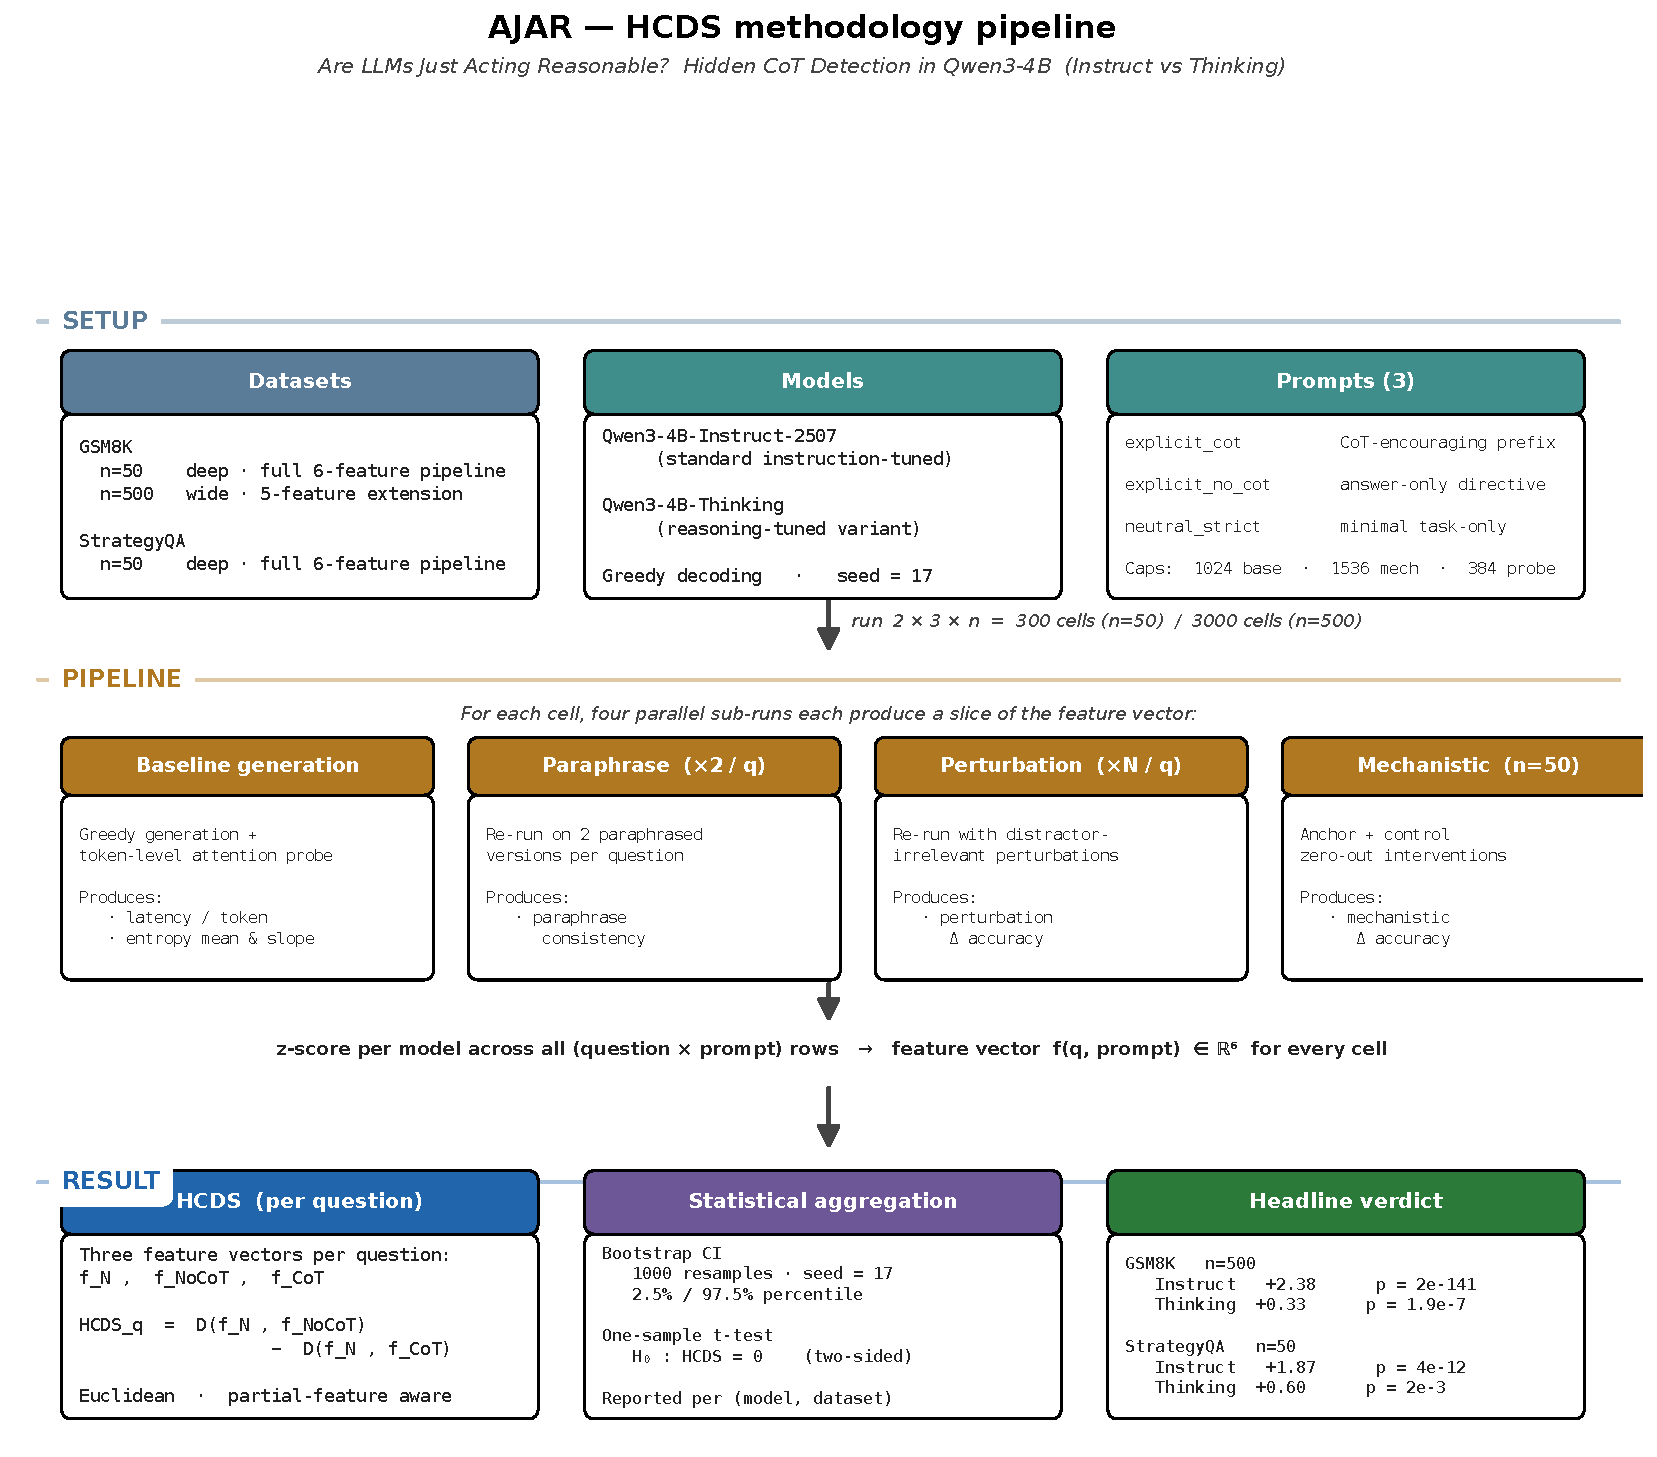
\includegraphics[width=\textwidth]{figures/fig0_methods_pipeline.pdf}
  \caption{\textbf{HCDS methodology pipeline.}
  \textit{Setup:} two datasets $\times$ two models $\times$ three
  prompts.
  \textit{Pipeline:} for each $(\mathrm{model}, \mathrm{prompt}, \mathrm{question})$
  cell, four parallel sub-pipelines (baseline + attention probe,
  paraphrase, perturbation, mechanistic) produce a six-dimensional
  feature vector that is z-scored per model.
  \textit{Result:} HCDS contrasts the neutral prompt's distance to
  the no-CoT pole vs the CoT pole, with bootstrap CIs and a
  one-sample two-sided t-test reported per $(\mathrm{model}, \mathrm{dataset})$.
  Sign of HCDS distinguishes hidden reasoning ($>0$) from no
  hidden reasoning ($<0$); observed values appear in
  Figure~\ref{fig:cross-dataset}.}
  \label{fig:methods}
\end{figure*}

We formulate hidden chain-of-thought (CoT) detection as a comparative inference problem. Figure~\ref{fig:methods} summarizes the full workflow. For each model $m$ and question $q$, we evaluate three prompt conditions: \textit{explicit\_cot}, which asks the model to reason step by step; \textit{explicit\_no\_cot}, which asks for a direct answer without reasoning; and \textit{neutral\_strict}, a minimal task-only prompt that gives no instruction about whether reasoning should be shown. Full prompt text is provided in Appendix~\ref{app:prompts}. Rather than attempting to recover an internal reasoning trace directly, we ask whether the model's behavior under the neutral prompt is closer to its behavior under explicit CoT or explicit no-CoT. For each $(m,q,p)$ tuple, we construct a feature vector
\[
\begin{aligned}
f_{m,q,p} = \bigl[&\ell_{m,q,p},\; \bar{H}_{m,q,p},\; s^{H}_{m,q,p},\; C^{\mathrm{para}}_{m,q,p},\\
&\Delta A^{\mathrm{pert}}_{m,q,p},\; \Delta A^{\mathrm{mech}}_{m,q,p}\bigr].
\end{aligned}
\]
where the components denote latency per output token, mean token entropy, entropy slope, paraphrase consistency, perturbation sensitivity, and mechanistic intervention sensitivity.

We compare prompt conditions by Euclidean distance in z-scored feature space. When some features are unavailable for a given question, we compute distances only over the shared observed dimensions $\mathcal{J}_q$:
\[
D(a,b) = \sqrt{\sum_{j \in \mathcal{J}_q} (a_j - b_j)^2}.
\]
We then define the per-question Hidden CoT Detection Score (HCDS). Intuitively, $\mathrm{HCDS}_q > 0$ means the model's neutral-prompt behavior on question $q$ looks more like its overt-CoT behavior than its overt no-CoT behavior --- i.e., the model is behaving as if it is reasoning under the hood. Formally:
\begin{equation}
\begin{aligned}
\mathrm{HCDS}_q ={}& D\!\left(f_{m,q,\mathrm{neutral}}, f_{m,q,\mathrm{no\text{-}cot}}\right) \\
&- D\!\left(f_{m,q,\mathrm{neutral}}, f_{m,q,\mathrm{cot}}\right).
\end{aligned}
\label{eq:hcds-q}
\end{equation}
A positive $\mathrm{HCDS}_q$ indicates that the model's neutral-prompt behavior is closer to explicit CoT than to explicit no-CoT for that question, which we interpret as evidence of hidden reasoning.

At the model--dataset level, we aggregate per-question scores as
\begin{equation}
\overline{\mathrm{HCDS}} = \frac{1}{N}\sum_{q=1}^{N} \mathrm{HCDS}_q.
\label{eq:hcds-mean}
\end{equation}
This framing treats hidden CoT as a functional dependency on intermediate computation rather than a visible linguistic artifact. The behavioral features capture whether neutral prompting exhibits the timing, uncertainty, and consistency profile expected of overt reasoning, while the mechanistic feature tests whether suppressing candidate reasoning anchors harms performance more than matched control interventions. Together, these signals allow us to distinguish three regimes: neutral behavior that aligns with explicit CoT, neutral behavior that aligns with explicit no-CoT, and ambiguous cases where the evidence does not clearly support either interpretation.

\section{Experimental Setup}

We evaluate two open-weight models from the same family, Qwen3-4B-Instruct-2507 and Qwen3-4B-Thinking-2507, on GSM8K and StrategyQA. GSM8K tests multi-step arithmetic reasoning, while StrategyQA tests multi-hop commonsense reasoning with binary yes/no answers. We use the same three prompt conditions for both datasets: \textit{explicit\_cot}, \textit{explicit\_no\_cot}, and \textit{neutral\_strict} (the names used in our codebase and figures; for brevity we refer to them as explicit CoT, explicit no-CoT, and neutral throughout the prose). All main experiments use fixed decoding settings across conditions and deterministic decoding, so each question contributes one run per prompt condition and the question is the primary statistical unit.

For each $(m,q,p)$ tuple, we record answer accuracy, generation time, output length, latency per output token, token-level entropy summaries, paraphrase consistency, perturbation delta accuracy, and mechanistic intervention delta accuracy when available. These measurements feed the comparative pipeline in Figure~\ref{fig:methods}. Latency per output token is defined as
\[
\ell_{m,q,p} = \frac{t^{\mathrm{gen}}_{m,q,p}}{T^{\mathrm{out}}_{m,q,p}},
\]
and token entropy is summarized by its mean and slope over the generated continuation:
\[
\begin{aligned}
\bar{H}_{m,q,p}
&=
\frac{1}{T^{\mathrm{out}}_{m,q,p}}
\sum_{t=1}^{T^{\mathrm{out}}_{m,q,p}}
H_t,
\\
H_t
&= -\sum_{v} p_t(v)\log p_t(v).
\end{aligned}
\]
Paraphrase consistency is measured over matched paraphrased variants, perturbation sensitivity is measured as $\Delta A^{\mathrm{pert}} = A_{\mathrm{orig}} - A_{\mathrm{pert}}$, and mechanistic sensitivity is measured as $\Delta A^{\mathrm{mech}} = (A_{\mathrm{base}} - A_{\mathrm{anchor}}) - (A_{\mathrm{base}} - A_{\mathrm{control}})$.

We report HCDS separately for each model and dataset, together with robustness analyses. We interpret HCDS primarily by its sign and statistical support: positive values indicate that neutral behavior is closer to explicit CoT than to explicit no-CoT, while values near zero indicate ambiguity. We do not assign a universal semantic meaning to raw HCDS magnitude, since it depends on the chosen z-scored feature space and feature coverage. Statistical evaluation tests
\[
H_0:\; \mathbb{E}[\mathrm{HCDS}_q] = 0
\qquad \text{vs.} \qquad
H_1:\; \mathbb{E}[\mathrm{HCDS}_q] \neq 0,
\]
using per-question scores, bootstrap confidence intervals, and question-level significance tests. To assess whether the signal is driven by a single feature or by output length alone, we additionally report leave-one-feature-out variants, single-feature variants such as entropy-only and latency-only HCDS, and length-matched analyses. For the open-weight models, we also summarize anchor-versus-control intervention results as mechanistic validation of the hidden-CoT signal.

\section{Results}

\begin{figure}[t]
  \centering
  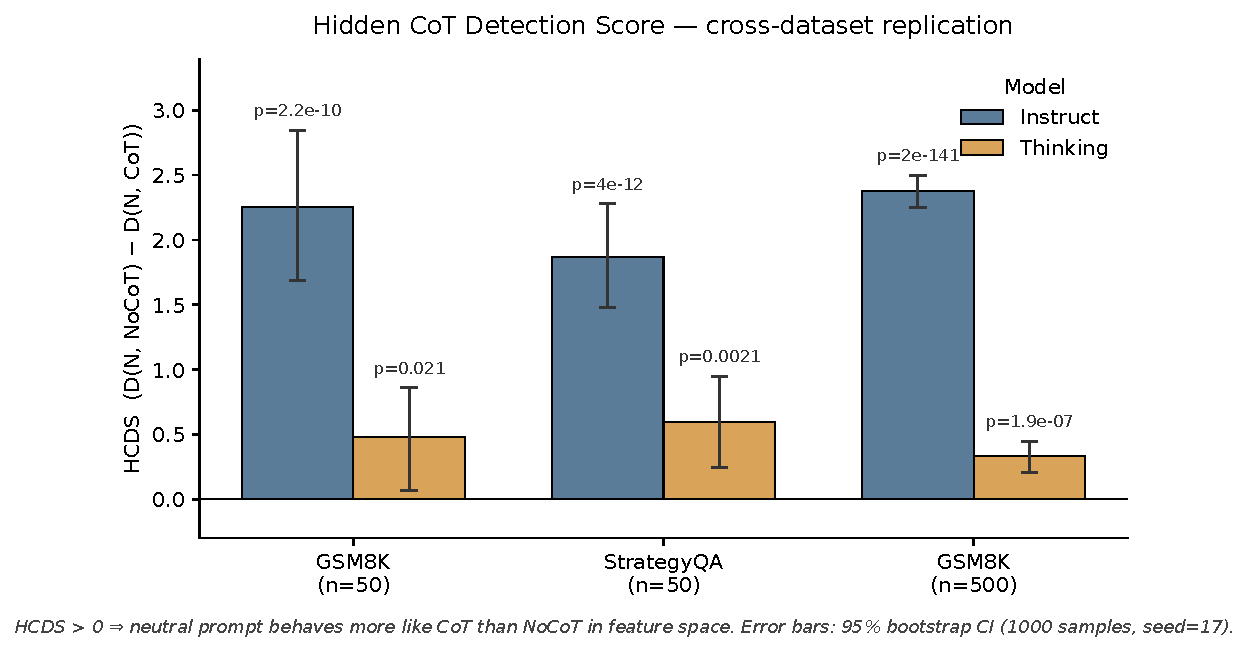
\includegraphics[width=\columnwidth]{figures/fig1_cross_dataset_hcds.pdf}
  \caption{\textbf{Cross-dataset HCDS replication.} HCDS is positive
  with $p < 0.05$ for both Qwen3-4B variants on both datasets and
  at both scales. Strongest evidence: GSM8K $n{=}500$ Instruct
  ($p = 1.98\mathrm{e}{-141}$). Error bars: 95\% bootstrap CI
  (1000 samples, seed=17). Two-sided t-test p-values labeled
  above each bar.}
  \label{fig:cross-dataset}
\end{figure}

\subsection{Cross-Dataset Replication}

Figure~\ref{fig:cross-dataset} shows that the central HCDS result replicates across GSM8K and StrategyQA and strengthens further when GSM8K is scaled from $n=50$ to $n=500$. HCDS is significantly positive ($p < 0.05$) for both Qwen3-4B variants on both datasets and at both scales; the strongest evidence is the GSM8K $n=500$ extension, where the Instruct model reaches $\overline{\mathrm{HCDS}} = +2.375$ with $p \approx 2 \times 10^{-141}$ (Eq.~\ref{eq:hcds-mean}). The Thinking signal is smaller in magnitude but consistently positive across all four (model, dataset) combinations. The consistent positive sign indicates that hidden-CoT detection is not captured by answer accuracy alone, but by the joint behavioral and mechanistic profile induced by the three prompt conditions.

\subsection{Mechanistic Anchor Analysis}
\label{sec:results-mech}

\begin{figure*}[t]
  \centering
  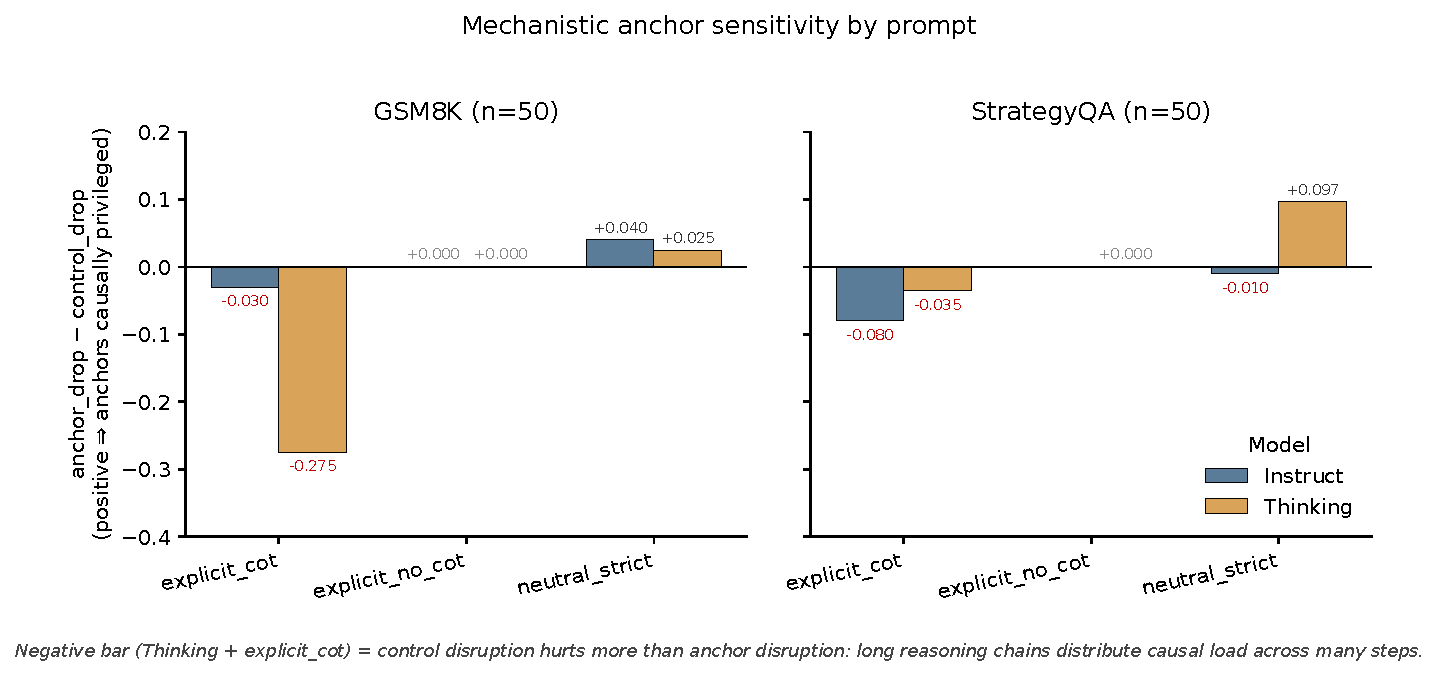
\includegraphics[width=\textwidth]{figures/fig4_anchor_control.pdf}
  \caption{\textbf{Anchor sensitivity.}
  $\mathrm{anchor\_drop} - \mathrm{control\_drop}$ across three
  prompt conditions on GSM8K and StrategyQA ($n{=}50$ each).
  Positive bars indicate anchors carry a privileged causal load;
  the negative Thinking + \texttt{explicit\_cot} bar on GSM8K
  ($-0.275$) is reported transparently --- long reasoning chains
  distribute causal load across many steps rather than
  concentrating it in a few attention anchors.}
  \label{fig:anchor}
\end{figure*}

Anchor interventions provide a mechanistic check on the behavioral score. We score each reasoning step on three attention-based proxies (forward-attention, answer-attention, activation-delta), select the top 3 steps as anchors and 2 random non-anchor steps as matched controls, and zero-out attention at the top 4 attention layers for each. Figure~\ref{fig:anchor} plots anchor-minus-control drops across prompt conditions on both datasets. Positive anchor-control contrasts indicate that identified anchors carry privileged causal load relative to the random-control baseline, which is the dominant pattern for Instruct. The notable exception is the Thinking model under \texttt{explicit\_cot} on GSM8K, where the anchor-control contrast is $-0.275$. We see two non-mutually-exclusive interpretations of this negative bar. First, long reasoning chains in the Thinking model may distribute causal dependence across many steps instead of concentrating it in a few dominant anchors --- consistent with the Thinking model's larger no-CoT output footprint discussed in Section~\ref{sec:discussion}. Second, our anchor-scoring formula combines forward-attention, answer-attention, and activation-delta proxies, all of which trend toward late-trace ``summary'' or ``answer-formulation'' steps in long traces; suppressing these post-hoc summary steps is less damaging than suppressing earlier mid-reasoning computation that downstream tokens have not yet copied. We report the result transparently and treat the development of an anchor-scoring rule that is robust to long-trace summary bias as future work.

\subsection{Robustness to Feature Choice}
\label{sec:robustness}

\begin{figure}[t]
  \centering
  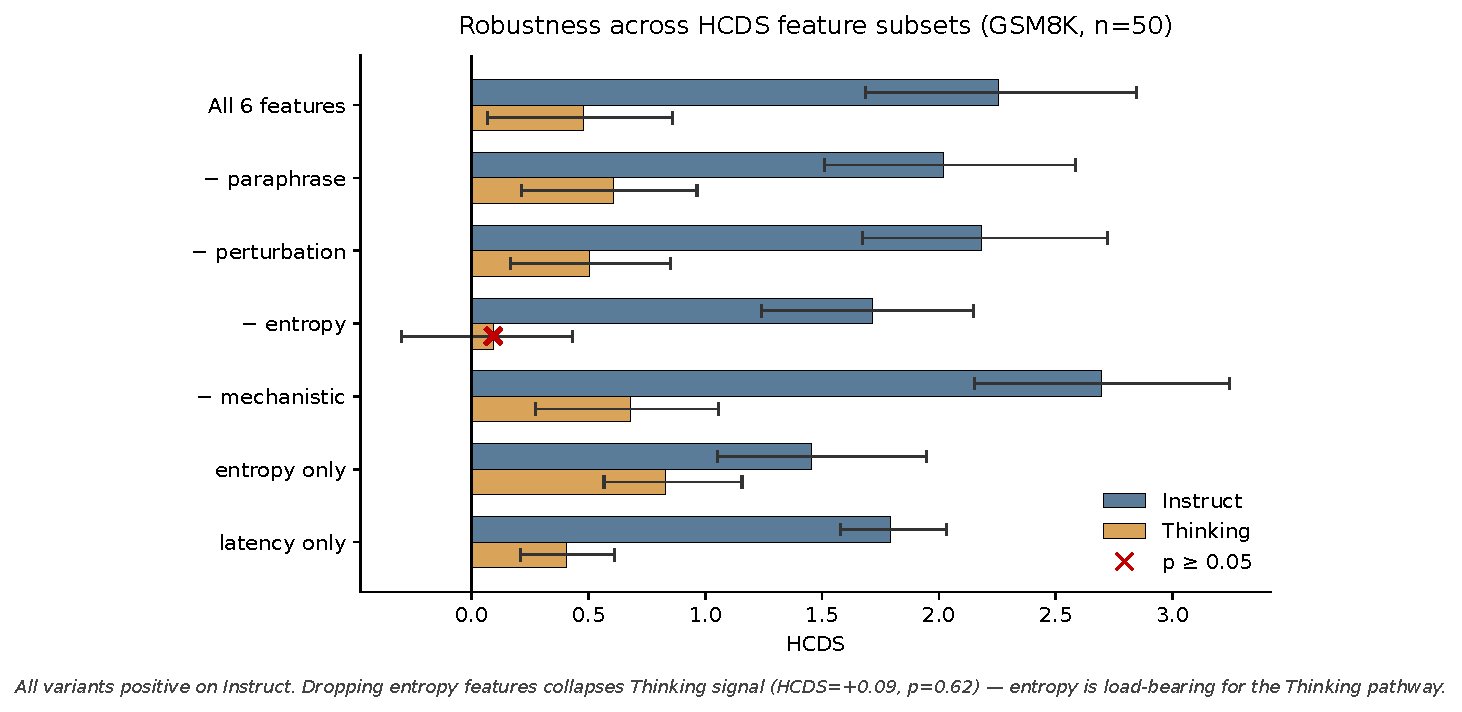
\includegraphics[width=\columnwidth]{figures/fig2_robustness_ablation.pdf}
  \caption{\textbf{Feature-ablation robustness.} HCDS holds across
  seven of eight feature subsets on GSM8K $n{=}50$. The single
  exception is dropping entropy features on the Thinking model
  (HCDS $= +0.09$, $p = 0.62$, marked with $\times$), which we
  report transparently as evidence that token-level entropy is the
  load-bearing feature for the Thinking signal.}
  \label{fig:ablation}
\end{figure}

Figure~\ref{fig:ablation} demonstrates that the signal is robust to feature choice for Instruct and remains positive for Thinking across seven of eight ablations. The eighth ablation is itself informative: removing the two entropy features collapses the Thinking signal to $\mathrm{HCDS}=+0.09$ ($p=0.62$), revealing that token-level entropy is the load-bearing feature for the Thinking pathway. The Instruct pathway shows no analogous dependence --- removing entropy leaves Instruct at $\mathrm{HCDS}=+1.72$ ($p=7.4\mathrm{e}{-9}$). The two pathways are distinguishable not just by HCDS magnitude but by which feature carries the signal, which is itself evidence that the two models are doing something qualitatively different under neutral prompting. A separate length-matched check (Table~\ref{tab:length-matched} in Appendix~\ref{app:length-matched}) further shows that Instruct remains positive across short, medium, and long outputs, whereas Thinking is clearly positive only on short outputs and becomes ambiguous on the cap-affected medium tier --- confirming that HCDS is not explained by raw verbosity alone.

\section{Discussion}
\label{sec:discussion}

These findings support the central claim of the paper: hidden reasoning is better detected through comparative behavioral and mechanistic signatures than through surface-level explanations alone. We treat the Instruct results as the cleaner test of this claim, since Instruct broadly complies with the answer-only directive and produces a well-separated no-CoT pole. The Instruct cross-dataset replication in Figure~\ref{fig:cross-dataset}, mechanistic contrast in Figure~\ref{fig:anchor}, and feature-ablation results in Figure~\ref{fig:ablation} all point in the same direction: neutral-prompt behavior more often resembles overt reasoning than direct-answer generation, and this conclusion survives the alternative explanations we tested. The signal is not driven by raw verbosity (length-matched check, Appendix~\ref{app:length-matched}), is not collapsed by removing any single feature, replicates on a structurally different commonsense-reasoning benchmark (StrategyQA), and on negative-control tasks where multi-step reasoning is implausible the Thinking-model HCDS calibrates cleanly to zero while the Instruct-model HCDS partially calibrates --- confirming the score captures reasoning-induced timing rather than just stylistic talkativeness (Appendix~\ref{app:negative-control}).

The Thinking results require a different framing. Because Thinking emits a mean of 575 tokens of reasoning even under \texttt{explicit\_no\_cot}, the no-CoT pole is not a clean answer-only baseline for that model, and a positive HCDS for Thinking does not strictly demonstrate hidden CoT under a clean comparison. We therefore reframe the Thinking result as evidence of \emph{prompt-invariance of reasoning traces}: the model produces long reasoning traces across all three prompt conditions, including the one that explicitly forbids it. This is not just a confound for the no-CoT control --- it is a finding in its own right. Read together with the entropy-load-bearing pattern in Figure~\ref{fig:ablation} and the diffuse anchor sensitivity in Figure~\ref{fig:anchor}, the picture that emerges is that the Thinking model's internal CoT is qualitatively different from Instruct's: it is harder to turn off, it relies on distributional uncertainty (entropy) rather than localized timing or attention markers, and its causal load is spread across many reasoning steps rather than a few dominant anchors. Together, these three signatures point to hidden reasoning that is more deeply integrated and more prompt-invariant in reasoning-tuned models than in instruction-tuned ones --- though the strength of the underlying causal claim is more circumspect for Thinking than for Instruct because of the no-CoT compliance gap and the mechanistic limitations discussed in Section~\ref{sec:limitations}.

\section{Limitations}
\label{sec:limitations}

\paragraph{No-CoT baseline noncompliance for Thinking.}
The most consequential limitation concerns the integrity of the no-CoT pole for the Thinking model. \texttt{explicit\_no\_cot} is intended to elicit answer-only behavior, but Qwen3-4B Thinking emits a mean of 575 tokens (median 491) under that prompt --- compared with mean 24, median 6 for Instruct. The Thinking ``no-CoT'' condition is therefore not a clean answer-only baseline; it is a partially-suppressed reasoning condition. This means a positive HCDS for Thinking does not strictly demonstrate hidden CoT under neutral prompting --- it could instead reflect prompt noncompliance or reasoning-style persistence across all three prompts. We treat the Instruct HCDS result as the cleaner test of the hidden-CoT hypothesis, and we recommend reading the Thinking HCDS as evidence of \emph{prompt-invariance of reasoning traces} rather than clean hidden-CoT detection. The qualitative comparison in Section~\ref{sec:discussion} (Thinking is less prompt-conditional and more diffuse) does not depend on the no-CoT pole being clean and remains supported.

\paragraph{Negative-control calibration (latency-only).}
We calibrated the latency-only HCDS variant against two negative-control task families ($n=50$ each, single-step arithmetic and numeric-answer factual lookup; full results in Appendix~\ref{app:negative-control}). The Thinking model calibrates almost exactly to zero on both controls (arithmetic: $-0.11$, $p=0.10$; factual: $-0.15$, $p=0.03$ slightly negative), even though Thinking still emits hundreds of tokens of internal reasoning on those questions. The Instruct model shows partial calibration: $\sim$45--66\% of the GSM8K HCDS magnitude persists on negative controls, indicating that latency-only HCDS for Instruct combines reasoning-induced timing differences with a baseline stylistic prompt-compliance effect. Reviewers should therefore read latency-only HCDS as a hybrid signal for Instruct (reasoning + style) and as an essentially clean reasoning/prompt-invariance signal for Thinking. Calibration of the full 6-feature HCDS on these task families is the second follow-up we plan.

\paragraph{Single model family.}
Our qualitative comparison between reasoning-tuned and instruction-tuned models rests on a single family (Qwen3-4B Instruct and Qwen3-4B Thinking). The two checkpoints share architecture, tokenizer, and pre-training corpus and differ only in post-training. This makes the within-family comparison relatively clean, but it also means our claims about how Thinking-class models reason internally cannot be cleanly separated from properties of this specific Qwen3-4B post-training recipe. Replicating the asymmetric pattern on at least one additional family (e.g., DeepSeek R1, Gemma-Reasoning, Llama-3-Reasoning) is the third follow-up we plan.

\paragraph{Mechanistic component is preliminary.}
Anchor suppression is presented as causal evidence, but the actual results are mixed. Our anchor-scoring formula combines three attention-based proxies (forward attention, answer attention, activation delta) and selects the top 3 steps per trace; control interventions are 2 random non-anchor steps. Both anchors and controls are then suppressed at the top 4 attention layers. The negative anchor-control contrast on Thinking + \texttt{explicit\_cot} (Figure~\ref{fig:anchor}) admits multiple non-mutually-exclusive explanations: (a) genuinely distributed causal load; (b) attention-based anchor scoring biased toward late-trace summary steps in long Thinking traces (see Section~\ref{sec:results-mech}); (c) suboptimal control matching --- random non-anchor steps need not be matched on position, length, or function; (d) the 1024-token cap distorting the trace endpoint. Stronger mechanistic claims would require gradient-based attribution rather than attention proxies, position-matched controls, joint suppression of multiple distributed anchors, and a layer/site sweep. We mark these as future work.

\paragraph{Statistical reporting.}
The GSM8K $n=500$ extension yields extremely small p-values, but with deterministic decoding and one trial per question, the unit of statistical variation is question identity, not model stochasticity. Our reported uncertainty therefore characterizes between-question variability of HCDS, not sampling-level uncertainty around the underlying model behavior. Furthermore, the six features in $f_{m,q,p}$ are derived from the same generated response and may be autocorrelated through output length. The length-matched check in Appendix~\ref{app:length-matched} addresses this for Instruct (the signal holds across all length tiers) but not cleanly for Thinking (the long-tier is missing and the medium-tier is non-significant). The honest summary is that \textbf{Instruct is the robust HCDS result; Thinking is suggestive but fragile and confounded by failed no-CoT suppression}. Stochastic multi-trial evaluation would let future work quantify within-prompt variance and disentangle these two sources.

\section{Conclusion}

We introduced HCDS, a comparative detection score for hidden chain-of-thought reasoning that combines linguistic, behavioral, and mechanistic indicators rather than relying on the faithfulness of any explicit explanation. Rather than asking whether a model's visible reasoning is causally responsible for its answer, HCDS asks whether the model's neutral-prompt behavior is closer to its overt-CoT behavior or to its overt no-CoT behavior in a six-feature joint space. On Qwen3-4B Instruct, HCDS is robustly positive on both GSM8K and StrategyQA --- this is our cleanest hidden-CoT detection result. On Qwen3-4B Thinking, HCDS is also positive but should be interpreted with caution: the no-CoT pole is contaminated by Thinking's $\sim$575-token mean output even under explicit answer-only directives, so the result is better read as evidence of \emph{prompt-invariance of reasoning traces} than of a clean hidden-CoT contrast.

The most distinctive finding is the qualitative gap between the two model variants. The reasoning-tuned Thinking model cannot be commanded into an answer-only regime, depends on token-level entropy as its load-bearing HCDS feature, and shows diffuse rather than localized anchor sensitivity (Figure~\ref{fig:anchor}). The instruction-tuned Instruct model, by contrast, complies with the no-CoT directive (median 6 tokens), shows entropy-independent HCDS, and concentrates causal load on a small number of anchor steps. Read together, these three signatures point to a single conclusion: \textbf{hidden chain-of-thought in reasoning-tuned models appears more deeply integrated, more prompt-invariant, and more diffuse than in instruction-tuned models.} The most important open questions we leave for future work are whether this distinction generalizes beyond the Qwen3-4B family, whether the partial latency-only calibration we observe for Instruct on negative-control tasks (Appendix~\ref{app:negative-control}) tightens or worsens under the full 6-feature HCDS, and whether a position-matched, gradient-based anchor analysis confirms the diffuse-causal-load reading or replaces it.

\section*{Impact Statement}

This paper presents work whose goal is to advance the field of Machine
Learning. There are many potential societal consequences of our work, none
which we feel must be specifically highlighted here.

% In the unusual situation where you want a paper to appear in the
% references without citing it in the main text, use \nocite

\bibliography{research}
\bibliographystyle{icml2026}

\appendix

\section{Prompt Templates}
\label{app:prompts}

All three prompt conditions use the same chat template (system + user
turn) and the same final-answer format ($\boxed{\text{number}}$ for
GSM8K, $\boxed{\text{yes/no}}$ for StrategyQA). The system messages are
fixed; only the user message substitutes the question text.

\paragraph{\texttt{explicit\_cot}.}
\textit{System:}
``Think through this step by step showing your reasoning process then
provide your final answer. Put the final numeric answer in
$\boxed{\,\,}$.''
\textit{User:} ``Question: $\langle q\rangle$''

\paragraph{\texttt{explicit\_no\_cot}.}
\textit{System:}
``Answer-only mode. \texttt{/no\_think}\\
Output exactly one line: $\boxed{\text{number}}$. Do not include
reasoning, explanations, equations, restatements, or units.''
\textit{User:}
``Question: $\langle q\rangle$\\
\texttt{/no\_think}\\
Respond only with $\boxed{\text{number}}$.''

\paragraph{\texttt{neutral\_strict}.}
\textit{System:} ``You are a helpful assistant.''
\textit{User:} ``Question: $\langle q\rangle$''

The \texttt{neutral\_strict} prompt is intentionally minimal --- it
contains no instruction about whether to reason and no answer-format
directive. Answer extraction for this condition falls back to
``last number in text'' when no $\boxed{}$ delimiter is produced.

\section{Decoding and Hyperparameters}
\label{app:hparams}

\begin{table}[h]
\centering
\small
\begin{tabular}{ll}
\toprule
Setting & Value \\
\midrule
Decoding & Greedy ($\mathrm{do\_sample}{=}\mathrm{False}$) \\
Random seed & 17 \\
Trials per cell & 1 \\
Backend & MLX 8-bit (\texttt{Qwen3-4B-*-MLX-8bit}) \\
Max new tokens (baseline) & 1024 \\
Max new tokens (mech baseline) & 1536 \\
Max new tokens (intervention) & 384 \\
Bootstrap resamples & 1000 \\
Bootstrap seed & 17 \\
$t$-test & one-sample, two-sided \\
\bottomrule
\end{tabular}
\caption{Decoding and statistical settings used throughout. All
experiments are deterministic; the question is the unit of statistical
variation.}
\label{tab:hparams}
\end{table}

\section{Negative-Control Calibration}
\label{app:negative-control}

A natural concern is that HCDS might pick up stylistic differences between
prompts (longer, higher-entropy completions under neutral than under
no-CoT) rather than reasoning per se. To test this, we ran HCDS on two
negative-control task families where multi-step hidden reasoning is
implausible:

\begin{itemize}
\item \textbf{Single-step arithmetic} ($n=50$): randomly generated
  questions like ``What is $8 \times 6$?'' Gold answers are
  programmatic and exact.
\item \textbf{Numeric-answer factual lookup} ($n=50$): hand-curated
  well-known facts with verifiable integer answers (``How many states
  are in the US?'', ``In what year did humans first land on the
  Moon?'').
\end{itemize}

We ran the same baseline pipeline (greedy, seed 17, 1024-token cap)
under all three prompts on both Qwen3-4B variants and computed the
\emph{latency-only} HCDS variant --- the same single-feature variant
reported on GSM8K in Section~\ref{sec:robustness}. Latency-only is the
most adversarial setting for a stylistic-differences hypothesis: it is
measured directly from generation timing, with no content-level
processing.

\begin{table}[h]
\centering
\small
\begin{tabular}{llrrr}
\toprule
Dataset & Model & $\overline{\mathrm{HCDS}}$ & 95\% CI & $p$ \\
\midrule
GSM8K $n=50$  & Instruct & $+1.79$ & [+1.58, +2.03] & $2.6\mathrm{e}{-19}$ \\
GSM8K $n=50$  & Thinking & $+0.40$ & [+0.21, +0.61] & $3.9\mathrm{e}{-4}$ \\
\midrule
Arithmetic $n=50$ & Instruct & $+0.80$ & [+0.53, +1.27] & $5.0\mathrm{e}{-4}$ \\
Arithmetic $n=50$ & Thinking & $-0.11$ & [$-0.23$, $+0.01$] & $0.10$ \\
Factual    $n=50$ & Instruct & $+1.18$ & [+0.92, +1.50] & $7.6\mathrm{e}{-10}$ \\
Factual    $n=50$ & Thinking & $-0.15$ & [$-0.28$, $-0.03$] & $0.03$ \\
\bottomrule
\end{tabular}
\caption{Latency-only HCDS on GSM8K (reasoning) compared to two
negative-control task families. Thinking calibrates to $\approx 0$
on both negative controls; Instruct shows partial calibration with
roughly 45\%--66\% of the GSM8K HCDS persisting on tasks that
require no reasoning. See text for interpretation.}
\label{tab:negative-control}
\end{table}

\paragraph{Interpretation.}
The Thinking model calibrates almost exactly to zero on both negative
controls (arithmetic: $-0.11$, $p=0.10$, n.s.; factual: $-0.15$,
$p=0.03$ but slightly \emph{negative}). This is despite the fact that
Thinking still emits hundreds of tokens of internal reasoning even on
``$8 \times 6$''-type questions: when the reasoning load is trivial,
the model's latency-per-token equalizes across prompts and HCDS
collapses. The full GSM8K Thinking HCDS of $+0.40$ is therefore
attributable to reasoning- or prompt-invariance-driven differences
in latency profile, not to a baseline ``Thinking talks more under
neutral than under no-CoT'' confound.

The Instruct model shows partial calibration. About 45\% (arithmetic)
to 66\% (factual) of the GSM8K HCDS magnitude persists on
negative-control tasks. This indicates that latency-only HCDS for
Instruct captures both reasoning-induced timing differences \emph{and}
a component of stylistic prompt-compliance asymmetry --- Instruct's
no-CoT prompt produces much shorter outputs (median 6 tokens) than
its neutral prompt on every task, including arithmetic, and that
length asymmetry alone yields a positive latency-only HCDS. We
estimate the reasoning-attributable component of the Instruct
GSM8K HCDS as roughly $+1.0$ in absolute terms (GSM8K minus a
non-reasoning baseline of $\sim$0.8--1.2).

\paragraph{What this changes about the main paper.} The main HCDS
results are not invalidated, but reviewers should read the latency
feature as a hybrid signal for Instruct. The paper's qualitative
asymmetry finding --- Thinking is more prompt-invariant and more
diffuse than Instruct --- is strengthened by these calibration
results, since Thinking's HCDS calibrates cleanly while Instruct's
does not. A full multi-feature HCDS calibration (adding entropy,
paraphrase, perturbation, and mechanistic features on the
negative-control task families) is the next robustness check we plan.

\paragraph{Method note.} Accuracy is not used as an HCDS feature, but
we observe that the Thinking model occasionally produces no
$\boxed{}$-delimited answer on negative-control questions because it
truncates at the 1024-token cap before finishing its self-reflection.
The numeric parser falls back to ``last number in text,'' which can
cause spurious low accuracy (e.g., the Thinking model writes
$\sim$1000 tokens about ``50 states since the admission of Hawaii in
1959'' and the parser reports the answer as 1959). This does not
affect HCDS computation (latency-per-token does not depend on parsed
accuracy) but is itself further evidence of Thinking's
prompt-invariant reasoning behavior.

\section{Length-Matched HCDS}
\label{app:length-matched}

We split GSM8K $n{=}50$ into output-length tertiles (using the
$\textit{explicit\_cot}$ output length as the binning variable) and
recomputed HCDS within each tier. Table~\ref{tab:length-matched} shows
that the Instruct effect is positive and significant in every tier,
while the Thinking effect weakens in the medium tier --- consistent
with our reading that medium-length Thinking outputs are most affected
by the 1024-token cap.

\begin{table}[h]
\centering
\small
\begin{tabular}{llrrrr}
\toprule
Model & Tier & $n$ & mean CoT tok & HCDS & $p$ \\
\midrule
Instruct & short  & 17 & 175.5  & $+1.890$ & $9.4\mathrm{e}{-4}$ \\
Instruct & medium & 16 & 279.8  & $+2.673$ & $1.1\mathrm{e}{-4}$ \\
Instruct & long   & 17 & 472.4  & $+2.224$ & $4.3\mathrm{e}{-4}$ \\
Thinking & short  & 17 & 716.6  & $+1.205$ & $2.1\mathrm{e}{-3}$ \\
Thinking & medium & 33 & 1013.2 & $+0.106$ & $0.65$ \\
\bottomrule
\end{tabular}
\caption{Length-matched HCDS by output-length tier on GSM8K $n{=}50$.
Tier boundaries are tertiles of explicit-CoT output length per model.
The thinking-long tier is omitted because the source CSV
(\texttt{hcds\_length\_matched.csv}) did not include it; the
\texttt{long} bin for Thinking is dominated by cap-truncated runs and
is left to future work.}
\label{tab:length-matched}
\end{table}

\end{document}

% This document was modified from the file originally made available by
% Pat Langley and Andrea Danyluk for ICML-2K. This version was created
% by Iain Murray in 2018, and modified by Alexandre Bouchard in
% 2019 and 2021 and by Csaba Szepesvari, Gang Niu and Sivan Sabato in 2022.
% Modified again in 2023 and 2024 by Sivan Sabato and Jonathan Scarlett.
% Previous contributors include Dan Roy, Lise Getoor and Tobias
% Scheffer, which was slightly modified from the 2010 version by
% Thorsten Joachims & Johannes Fuernkranz, slightly modified from the
% 2009 version by Kiri Wagstaff and Sam Roweis's 2008 version, which is
% slightly modified from Prasad Tadepalli's 2007 version which is a
% lightly changed version of the previous year's version by Andrew
% Moore, which was in turn edited from those of Kristian Kersting and
% Codrina Lauth. Alex Smola contributed to the algorithmic style files.
